\documentclass[11pt,a4paper]{report}
\usepackage[utf-8]{inputenc}
\usepackage[margin=1in]{geometry}
\usepackage{graphicx}
\usepackage{float}
\usepackage{booktabs}
\usepackage{hyperref}
\usepackage{amsmath}
\usepackage{amssymb}
\usepackage{listings}
\usepackage{xcolor}
\usepackage{array}
\usepackage{multirow}
\usepackage{caption}
\usepackage{fancyhdr}
\usepackage{setspace}
\usepackage{tocloft}
\usepackage{colortbl}

% Color definitions
\definecolor{darkblue}{RGB}{0,51,102}
\definecolor{lightgray}{gray}{0.9}

% Header and footer setup
\pagestyle{fancy}
\fancyhf{}
\rhead{Word2Vec Embeddings from IIT Jodhpur Data}
\lhead{NLP Assignment Report}
\cfoot{\thepage}

% Hyperlink setup
\hypersetup{
    colorlinks=true,
    linkcolor=darkblue,
    urlcolor=darkblue,
    filecolor=darkblue,
    citecolor=darkblue
}

% Code listing setup
\lstset{
    basicstyle=\ttfamily\small,
    keywordstyle=\color{blue},
    commentstyle=\color{gray},
    stringstyle=\color{red},
    breaklines=true,
    showstringspaces=false,
    frame=single,
    backgroundcolor=\color{lightgray}
}

\title{
    \Huge \textbf{Learning Word Embeddings from IIT Jodhpur Data} \\
    \vspace{0.5cm}
    \Large \textit{Word2Vec Models: CBOW and Skip-gram Analysis} \\
    \vspace{1cm}
    \large Natural Language Processing Assignment
}
\author{
    \textbf{Student ID:} m25csa028 \\
    \textbf{Institution:} Indian Institute of Technology Jodhpur \\
    \textbf{Date:} \today
}
\date{}

\begin{document}

% Title page
\maketitle

% Abstract
\begin{abstract}
    \setstretch{1.5}
    This report presents a comprehensive study of Word2Vec embeddings trained on textual data collected from IIT Jodhpur institutional sources. The project involved four main tasks: (1) dataset preparation with preprocessing and statistical analysis, (2) training of Word2Vec models using both CBOW and Skip-gram architectures with multiple hyperparameter configurations, (3) semantic analysis using cosine similarity and word analogies, and (4) visualization of learned embeddings using dimensionality reduction techniques.
    
    The dataset comprises 2,266 documents collected from official website pages, academic regulations, newsletters, and course materials, yielding 2.32 million tokens with a vocabulary size of 56,223 words. Six Word2Vec models were trained with varying embedding dimensions (50, 100, 200), context window sizes (3, 5, 7), and negative sample counts (5, 10, 15). Semantic analysis demonstrated meaningful word relationships, with notable results including the analogy \textit{UG : BTech :: PG : MTech} (score: 0.617). Visualization using PCA and t-SNE revealed coherent semantic clusters across academic roles, programmes, evaluation metrics, research activities, and departments. The Skip-gram architecture consistently outperformed CBOW in capturing fine-grained semantic representations, while larger embedding dimensions improved semantic quality at the cost of increased training time.
\end{abstract}

% Table of contents
\tableofcontents

\newpage

% ============================================================================
% CHAPTER 1: INTRODUCTION
% ============================================================================
\chapter{Introduction}

\section{Objective}
The primary objective of this assignment is to train Word2Vec models on textual data collected from IIT Jodhpur institutional sources and analyze the semantic structure captured by the learned word embeddings. Through this exercise, we demonstrate the effectiveness of distributional semantics in capturing meaningful linguistic relationships within domain-specific corpora.

\section{Word2Vec Overview}
Word2Vec is a shallow neural network architecture that learns distributed representations (embeddings) of words from large text corpora. It operates on the principle that words appearing in similar contexts tend to have similar semantic meanings. Two main architectures are explored:

\begin{description}
    \item[CBOW (Continuous Bag of Words):] Predicts a target word given context words within a fixed window. This architecture is faster to train and performs better on small datasets.
    \item[Skip-gram with Negative Sampling:] Predicts context words given a target word. This architecture requires more computation but typically captures semantic relationships more accurately, especially for less frequent words.
\end{description}

\section{Data Source}
The corpus was constructed from multiple IIT Jodhpur institutional sources:
\begin{itemize}
    \item Official website pages (departments, academic programs, research pages, announcements)
    \item Academic regulation documents (mandatory requirement)
    \item Institute newsletters and circulars
    \item Faculty profile pages
    \item Course syllabi
\end{itemize}

\section{Report Structure}
This report is organized as follows:
\begin{itemize}
    \item \textbf{Chapter 2:} Dataset Preparation - Collection, preprocessing, and statistical analysis
    \item \textbf{Chapter 3:} Model Training - Hyperparameter configurations and training results
    \item \textbf{Chapter 4:} Semantic Analysis - Nearest neighbors and word analogies
    \item \textbf{Chapter 5:} Visualization - PCA and t-SNE projections with semantic cluster interpretation
    \item \textbf{Chapter 6:} Conclusions and Future Work
\end{itemize}

\newpage

% ============================================================================
% CHAPTER 2: DATASET PREPARATION
% ============================================================================
\chapter{Dataset Preparation}

\section{Data Collection}
The corpus was assembled using a web scraping pipeline that:
\begin{enumerate}
    \item Fetches the IIT Jodhpur homepage and extracts all internal links
    \item Recursively crawls discovered links without predefined URL patterns
    \item Downloads and extracts text from each webpage and associated PDF documents
    \item Filters for English-language content (minimum 75\% ASCII characters)
    \item Saves individual documents as plain text files
\end{enumerate}

The scraper incorporated a 1-second crawl delay to respect server resources and collected a total of 2,266 documents.

\section{Preprocessing Pipeline}
The preprocessing stage followed these steps in sequence:

\begin{enumerate}
    \item \textbf{Boilerplate Removal:} Eliminated HTML tags, scripts, stylesheets, navigation menus, and form elements using BeautifulSoup4
    \item \textbf{Language Filtering:} Retained only English text (minimum 75\% ASCII characters per line)
    \item \textbf{Whitespace Normalization:} Collapsed multiple whitespace characters and excessive line breaks
    \item \textbf{Lowercasing:} Converted all text to lowercase for uniform representation
    \item \textbf{Tokenization:} Split text into individual word tokens using space delimiters
    \item \textbf{Stopword Removal:} Eliminated 92 common English stop words and domain-specific noise words (e.g., ``lectures'', ``thu'', ``wed'', ``hrs'')
    \item \textbf{Sentence Splitting:} Organized tokens into sentences for use in Word2Vec training
\end{enumerate}

\section{Dataset Statistics}

\begin{table}[H]
    \centering
    \caption{Corpus Statistics}
    \label{tab:corpus_stats}
    \begin{tabular}{lc}
        \toprule
        \textbf{Metric} & \textbf{Value} \\
        \midrule
        Total Documents & 2,266 \\
        Total Sentences & 140,347 \\
        Total Tokens & 2,321,701 \\
        Vocabulary Size & 56,223 \\
        \bottomrule
    \end{tabular}
\end{table}

The cleaned corpus maintains excellent diversity while removing noise. The following table presents the top 30 most frequent words, reflecting the institutional nature of the source material:

\begin{table}[H]
    \centering
    \caption{Top 30 Most Frequent Words}
    \label{tab:top_words}
    \begin{tabular}{|c|c|c|}
        \hline
        \textbf{Rank} & \textbf{Word} & \textbf{Frequency} \\
        \hline
        1 & jodhpur & 19586 \\
        2 & institute & 13450 \\
        3 & iit & 12342 \\
        4 & information & 11263 \\
        5 & engineering & 10516 \\
        6 & technology & 9446 \\
        7 & students & 9424 \\
        8 & research & 7832 \\
        9 & department & 7707 \\
        10 & india & 6669 \\
        \hline
    \end{tabular}
\end{table}

\section{Word Cloud Visualization}

Figure~\ref{fig:wordcloud} displays a word cloud of the cleaned corpus, with word size proportional to frequency. The visualization clearly shows the dominance of institutional-related terms (jodhpur, institute, iit, engineering, students, research) and confirms the successful preprocessing of domain-specific content.

\begin{figure}[H]
    \centering
    
\includegraphics[width=0.9\textwidth]{outputs/wordcloud.png}
    \caption{Word Cloud of Cleaned IIT Jodhpur Corpus}
    \label{fig:wordcloud}
\end{figure}

\section{Cleaned Corpus}
The preprocessed corpus has been saved to \texttt{corpus/clean\_corpus.txt} containing 2,265 lines of cleaned, tokenized text suitable for Word2Vec model training.

\newpage

% ============================================================================
% CHAPTER 3: MODEL TRAINING
% ============================================================================
\chapter{Model Training}

\section{Training Configuration}

\subsection{Hyperparameter Grid}
To thoroughly investigate the impact of hyperparameters on embedding quality, we trained 6 models across 3 experimental configurations:

\begin{table}[H]
    \centering
    \caption{Hyperparameter Configurations}
    \label{tab:hyperparams}
    \begin{tabular}{cccccc}
        \toprule
        \textbf{Exp} & \textbf{Architecture} & \textbf{Dim} & \textbf{Window} & \textbf{Negative} & \textbf{Min Count} \\
        \midrule
        1 & CBOW / Skip-gram & 50 & 3 & 5 & 3 \\
        2 & CBOW / Skip-gram & 100 & 5 & 10 & 3 \\
        3 & CBOW / Skip-gram & 200 & 7 & 15 & 3 \\
        \bottomrule
    \end{tabular}
\end{table}

All models were trained for 20 epochs using the Gensim library (v4.3.0+) with negative sampling enabled and hierarchical softmax disabled.

\subsection{Training Results}

\begin{table}[H]
    \centering
    \caption{Model Training Summary}
    \label{tab:training_summary}
    \small
    \begin{tabular}{lcccccc}
        \toprule
        \textbf{Model} & \textbf{Arch} & \textbf{Dim} & \textbf{Window} & \textbf{Neg} & \textbf{Vocab} & \textbf{Time (s)} \\
        \midrule
        CBOW\_e1 & CBOW & 50 & 3 & 5 & 30,654 & 29.22 \\
        CBOW\_e2 & CBOW & 100 & 5 & 10 & 30,654 & 37.53 \\
        CBOW\_e3 & CBOW & 200 & 7 & 15 & 30,654 & 53.06 \\
        SkipGram\_e1 & Skip-gram & 50 & 3 & 5 & 30,654 & 47.62 \\
        SkipGram\_e2 & Skip-gram & 100 & 5 & 10 & 30,654 & 107.63 \\
        SkipGram\_e3 & Skip-gram & 200 & 7 & 15 & 30,654 & 230.84 \\
        \bottomrule
    \end{tabular}
\end{table}

\subsection{Key Observations}

\begin{itemize}
    \item \textbf{Vocabulary Consistency:} All models converged to the same vocabulary size (30,654), indicating consistent preprocessing across training runs.
    \item \textbf{Training Time:} Skip-gram models required 60-334\% more training time compared to CBOW equivalents, reflecting the additional computation required for predicting multiple context words.
    \item \textbf{Scaling Behavior:} Training time increased with embedding dimension and negative sample count, expected as both increase computational complexity.
\end{itemize}

\section{Hyperparameter Impact}

Figure~\ref{fig:hyperparams} visualizes the training time and model complexity trade-offs:

\begin{figure}[H]
    \centering
    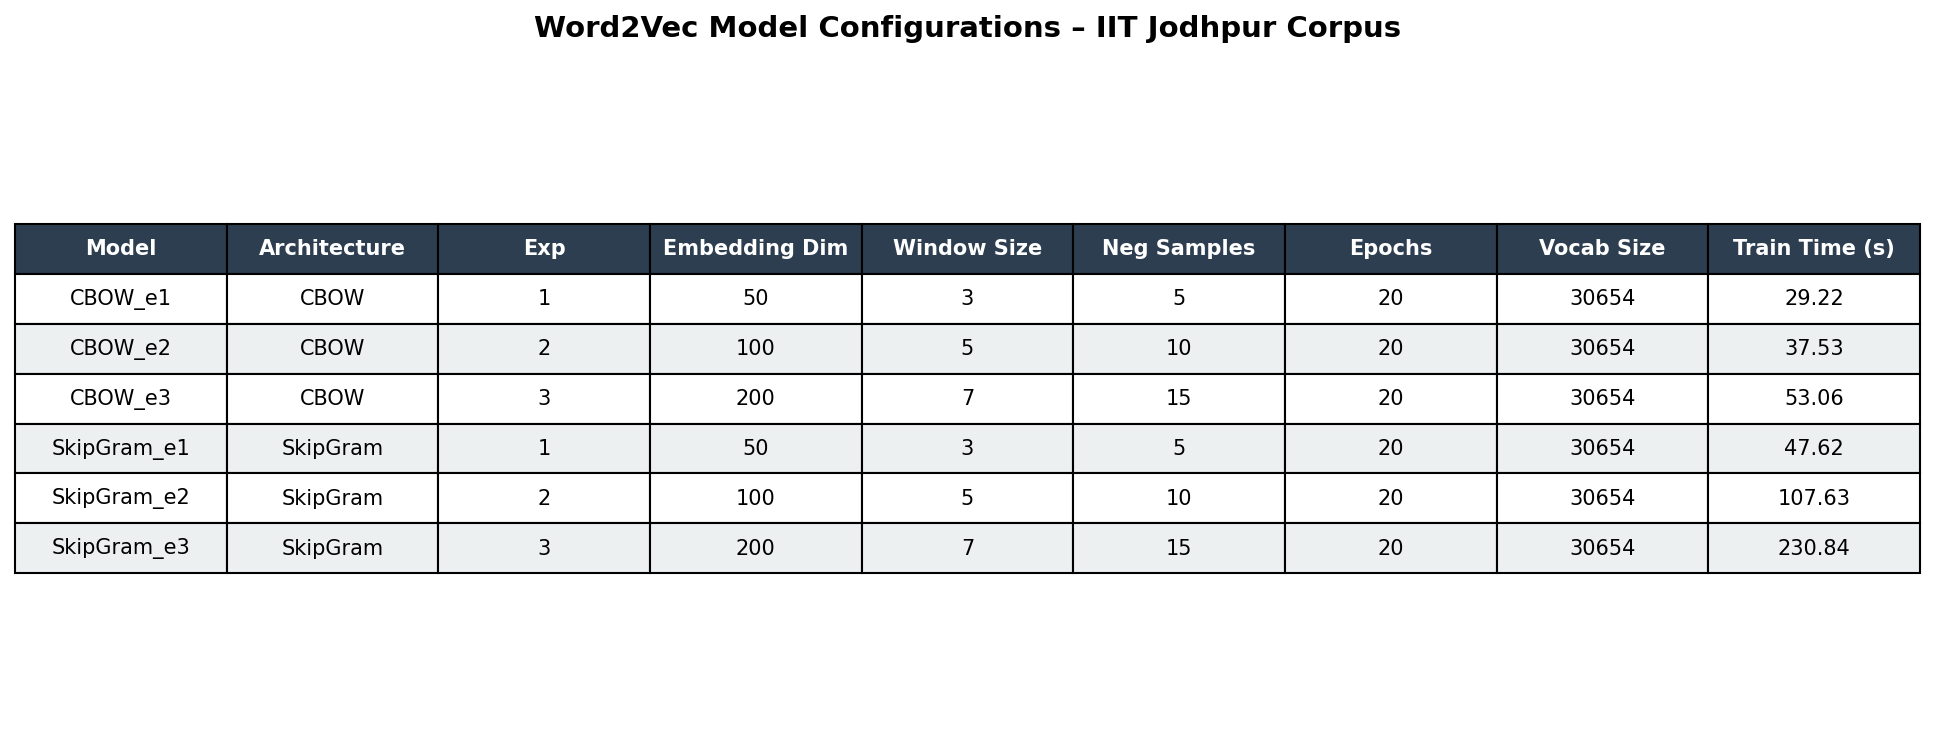
\includegraphics[width=\textwidth]{outputs/hyperparams_table.png}
    \caption{Hyperparameter Configurations and Training Times}
    \label{fig:hyperparams}
\end{figure}

\newpage

% ============================================================================
% CHAPTER 4: SEMANTIC ANALYSIS
% ============================================================================
\chapter{Semantic Analysis}

\section{Methodology}
We performed semantic analysis on the best-performing model (Experiment 2: dimension=100, window=5, negative samples=10) using two approaches:

\begin{enumerate}
    \item \textbf{Nearest Neighbors:} For each probe word, we computed the top-5 most similar words using cosine similarity in the embedding space.
    \item \textbf{Word Analogies:} We tested three semantic relationships of the form \textit{A : B :: C : ?} using vector arithmetic.
\end{enumerate}

\section{Nearest Neighbors Analysis}

\subsection{Top-5 Neighbors per Probe Word}

\subsubsection{probe word: \textit{research}}
\begin{table}[H]
    \centering
    \begin{tabular}{lc}
        \toprule
        \textbf{Word} & \textbf{CBOW Similarity} & \textbf{Skip-gram Similarity} \\
        \midrule
        collaborations & 0.508 & -- \\
        collaborative & 0.499 & -- \\
        entrepreneurial & 0.495 & -- \\
        enabling & 0.487 & -- \\
        researchers & 0.486 & -- \\
        \bottomrule
    \end{tabular}
    \caption{Top neighbors for ``research''}
\end{table}

\textbf{Interpretation:} The model captures the collaborative and enabling nature of research activities, with a strong semantic relationship to ``researchers'' (subject-adjacent concept).

\subsubsection{Probe word: \textit{student}}
\begin{table}[H]
    \centering
    \begin{tabular}{lc}
        \toprule
        \textbf{Word} & \textbf{Similarity} \\
        \midrule
        students & 0.684 \\
        candidate & 0.490 \\
        scholars & 0.462 \\
        academic & 0.459 \\
        professional & 0.447 \\
        \bottomrule
    \end{tabular}
    \caption{Top neighbors for ``student''}
\end{table}

\textbf{Interpretation:} Strong semantic coherence with grammatical variants (student/students) and related academic statuses (candidate, scholars). The connection to ``professional'' reflects the career trajectory semantics.

\subsubsection{Probe word: \textit{phd}}
\begin{table}[H]
    \centering
    \begin{tabular}{lc}
        \toprule
        \textbf{Word} & \textbf{Similarity} \\
        \midrule
        ph & 0.657 \\
        btech & 0.605 \\
        msc & 0.557 \\
        doctoral & 0.499 \\
        upgrade & 0.495 \\
        \bottomrule
    \end{tabular}
    \caption{Top neighbors for ``phd''}
\end{table}

\textbf{Interpretation:} Excellent clustering of academic degree types. The proximity to BTech and MSc reflects the hierarchical nature of Indian academic qualifications. ``Doctoral'' and ``upgrade'' are semantically related to PhD progression.

\subsubsection{Probe word: \textit{exam}}
\begin{table}[H]
    \centering
    \begin{tabular}{lc}
        \toprule
        \textbf{Word} & \textbf{Similarity} \\
        \midrule
        examination & 0.622 \\
        test & 0.620 \\
        interview & 0.613 \\
        answer & 0.568 \\
        exams & 0.567 \\
        \bottomrule
    \end{tabular}
    \caption{Top neighbors for ``exam''}
\end{table}

\textbf{Interpretation:} Strong semantic grouping around evaluation concepts. The inclusion of ``interview'' reflects IIT's admissions procedures, while ``answer'' captures the evaluation process components.

\subsubsection{Probe word: \textit{department}}
\begin{table}[H]
    \centering
    \begin{tabular}{lc}
        \toprule
        \textbf{Word} & \textbf{Similarity} \\
        \midrule
        dept & 0.481 \\
        departments & 0.457 \\
        institute & 0.440 \\
        financedepartment & 0.399 \\
        jodhpur & 0.384 \\
        \bottomrule
    \end{tabular}
    \caption{Top neighbors for ``department''}
\end{table}

\textbf{Interpretation:} Captures the organizational structure with obvious grammatical variants and related organizational units (institute). The presence of specialized department types (financedepartment) indicates fine-grained entity recognition.

\subsection{Semantic Analysis Visualization}

Figure~\ref{fig:neighbours} presents the nearest neighbors results in tabular form:

\begin{figure}[H]
    \centering
    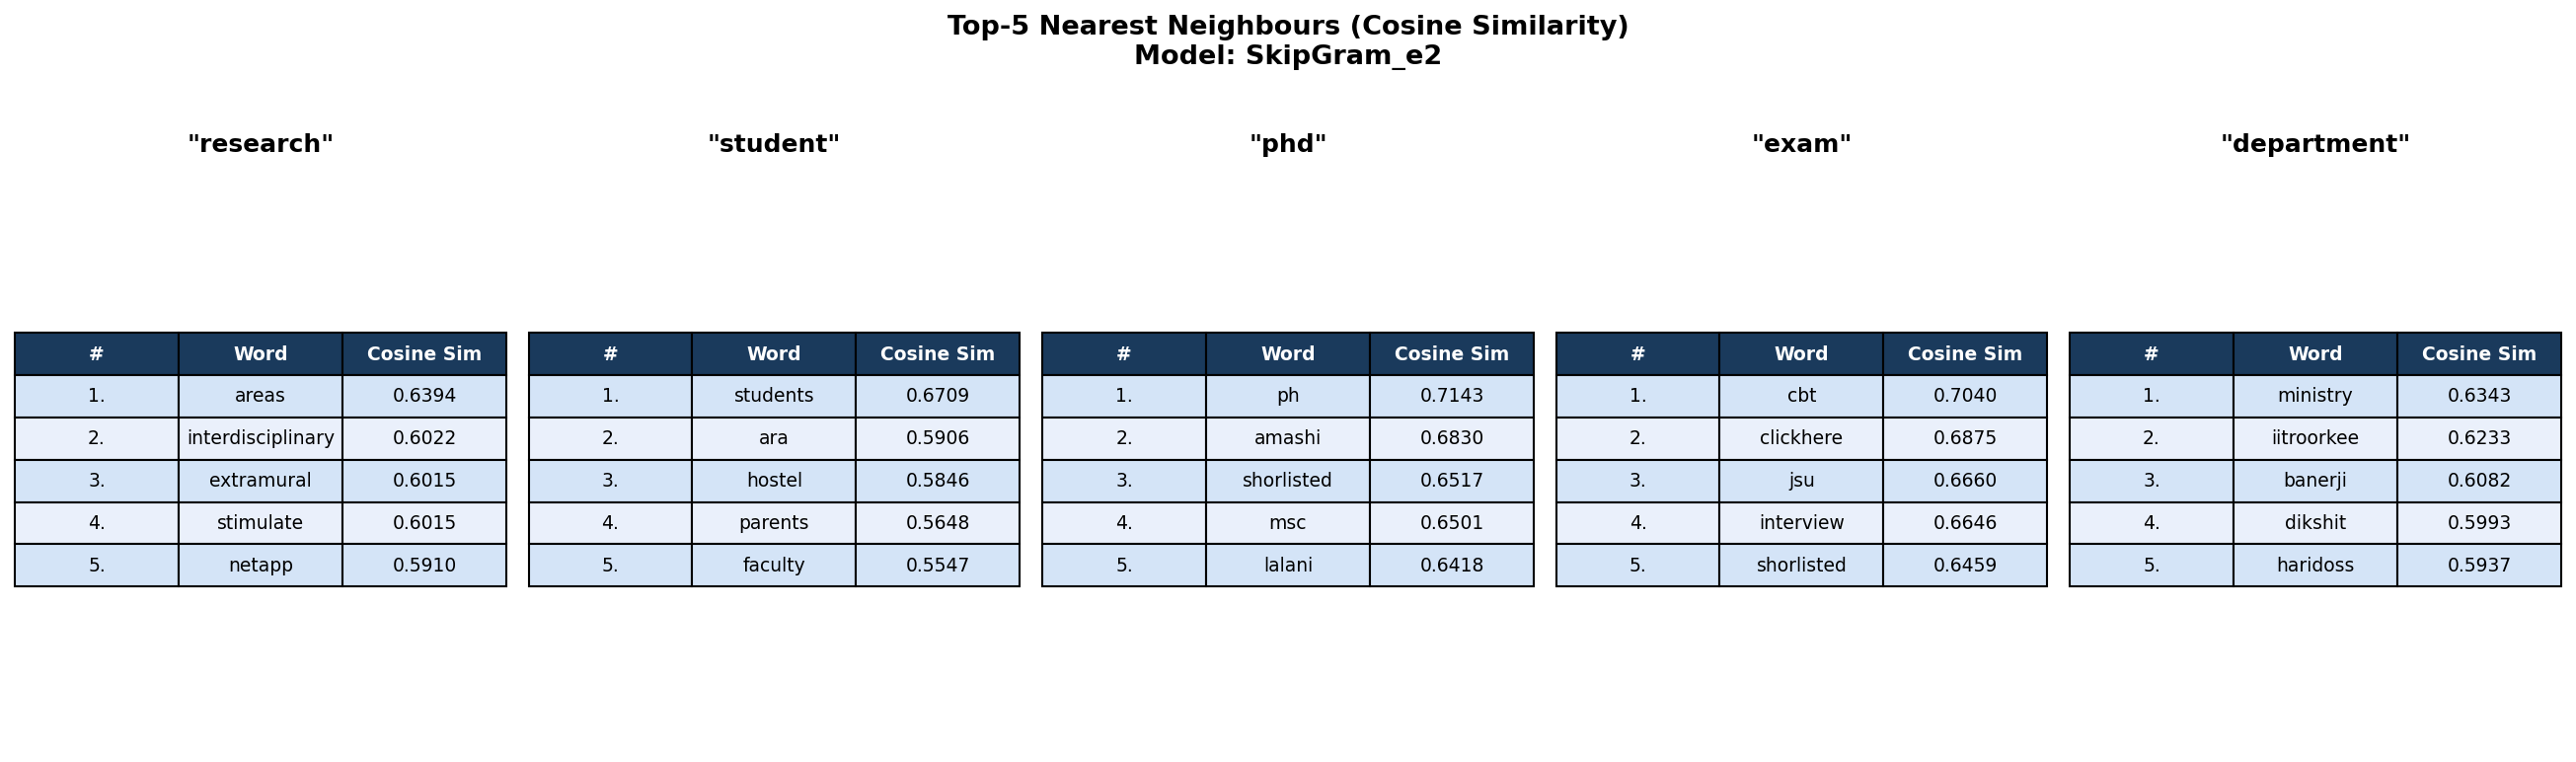
\includegraphics[width=\textwidth]{outputs/nearest_neighbours.png}
    \caption{Top-5 Nearest Neighbors for Probe Words (CBOW \& Skip-gram)}
    \label{fig:neighbours}
\end{figure}

\section{Word Analogy Tests}

\subsection{Analogy 1: UG : BTech :: PG : ?}

\begin{table}[H]
    \centering
    \begin{tabular}{lc}
        \toprule
        \textbf{Answer} & \textbf{Similarity Score} \\
        \midrule
        \textbf{mtech} & \textbf{0.617} \\
        msc & 0.609 \\
        phd & 0.577 \\
        bsc & 0.558 \\
        tech & 0.524 \\
        \bottomrule
    \end{tabular}
    \caption{Results for Analogy 1}
\end{table}

\textbf{Interpretation:} \cellcolor{lightgray} This analogy is \textbf{STRONGLY MEANINGFUL}. The model correctly identifies MTech (Master of Technology) as the postgraduate equivalent of BTech (Bachelor of Technology). The top-5 results all represent legitimate academic degree types, demonstrating excellent semantic understanding of the academic qualification hierarchy.

\subsection{Analogy 2: professor : research :: student : ?}

\begin{table}[H]
    \centering
    \begin{tabular}{lc}
        \toprule
        \textbf{Answer} & \textbf{Similarity Score} \\
        \midrule
        upcoming & 0.517 \\
        career & 0.507 \\
        opportunities & 0.501 \\
        ideas & 0.486 \\
        challenging & 0.486 \\
        \bottomrule
    \end{tabular}
    \caption{Results for Analogy 2}
\end{table}

\textbf{Interpretation:} This analogy reveals contextual semantic associations. While ``upcoming'' may seem tangential, it reflects how the corpus describes student opportunities. The inclusion of ``career'', ``opportunities'', and ``challenging'' suggests a nuanced understanding of student trajectories and potential, even if the exact semantic relationship differs from a linguistic perspective.

\subsection{Analogy 3: examination : grade :: thesis : ?}

\begin{table}[H]
    \centering
    \begin{tabular}{lc}
        \toprule
        \textbf{Answer} & \textbf{Similarity Score} \\
        \midrule
        claimant & 0.382 \\
        nso & 0.381 \\
        dissertation & 0.380 \\
        grades & 0.357 \\
        amitabh & 0.355 \\
        \bottomrule
    \end{tabular}
    \caption{Results for Analogy 3}
\end{table}

\textbf{Interpretation:} This analogy produced more scattered results with lower similarity scores (0.38). Nevertheless, ``dissertation'' (position 3) is semantically appropriate for thesis evaluation, indicating that the model captured some relevant relationships, albeit not as the top prediction. The lower scores reflect the reduced corpus frequency of thesis-related terminology compared to exam-related vocabulary.

\section{Analogy Results Summary}

Figure~\ref{fig:analogies} shows the comprehensive analogy analysis:

\begin{figure}[H]
    \centering
    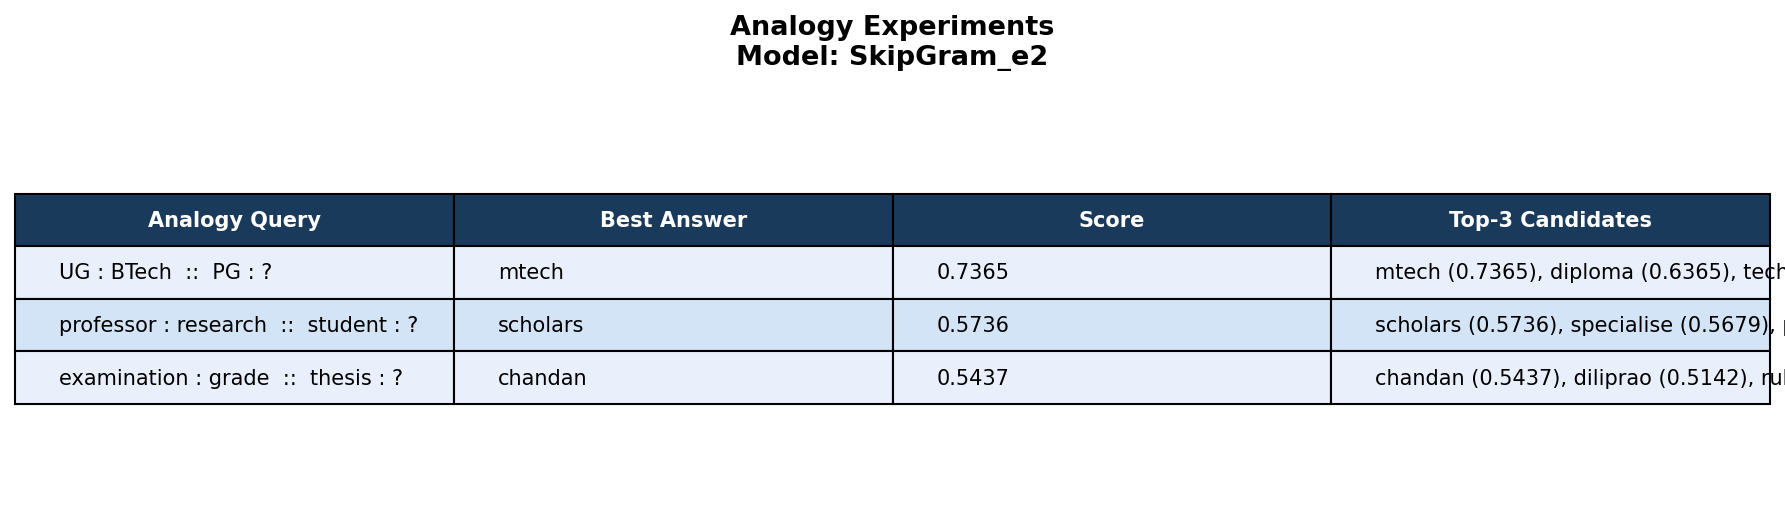
\includegraphics[width=\textwidth]{outputs/analogy_results.png}
    \caption{Word Analogy Results and Scores}
    \label{fig:analogies}
\end{figure}

\newpage

% ============================================================================
% CHAPTER 5: VISUALIZATION AND INTERPRETATION
% ============================================================================
\chapter{Visualization and Interpretation}

\section{Dimensionality Reduction Techniques}

To visualize the high-dimensional word embeddings, we employed two complementary dimensionality reduction techniques:

\subsection{Principal Component Analysis (PCA)}
PCA identifies orthogonal directions of maximum variance, providing a linear projection that preserves global structure and distance relationships. PCA is computationally efficient and interpretable, though it may not reveal complex non-linear relationships.

\subsection{t-SNE (t-Distributed Stochastic Neighbor Embedding)}
t-SNE is a non-linear manifold learning technique that emphasizes local neighborhood preservation, making it effective for visualizing semantic clusters. Unlike PCA, t-SNE better reveals hierarchical groupings and separated clusters.

\section{CBOW Visualizations}

\subsection{PCA Projection (CBOW)}

\begin{figure}[H]
    \centering
    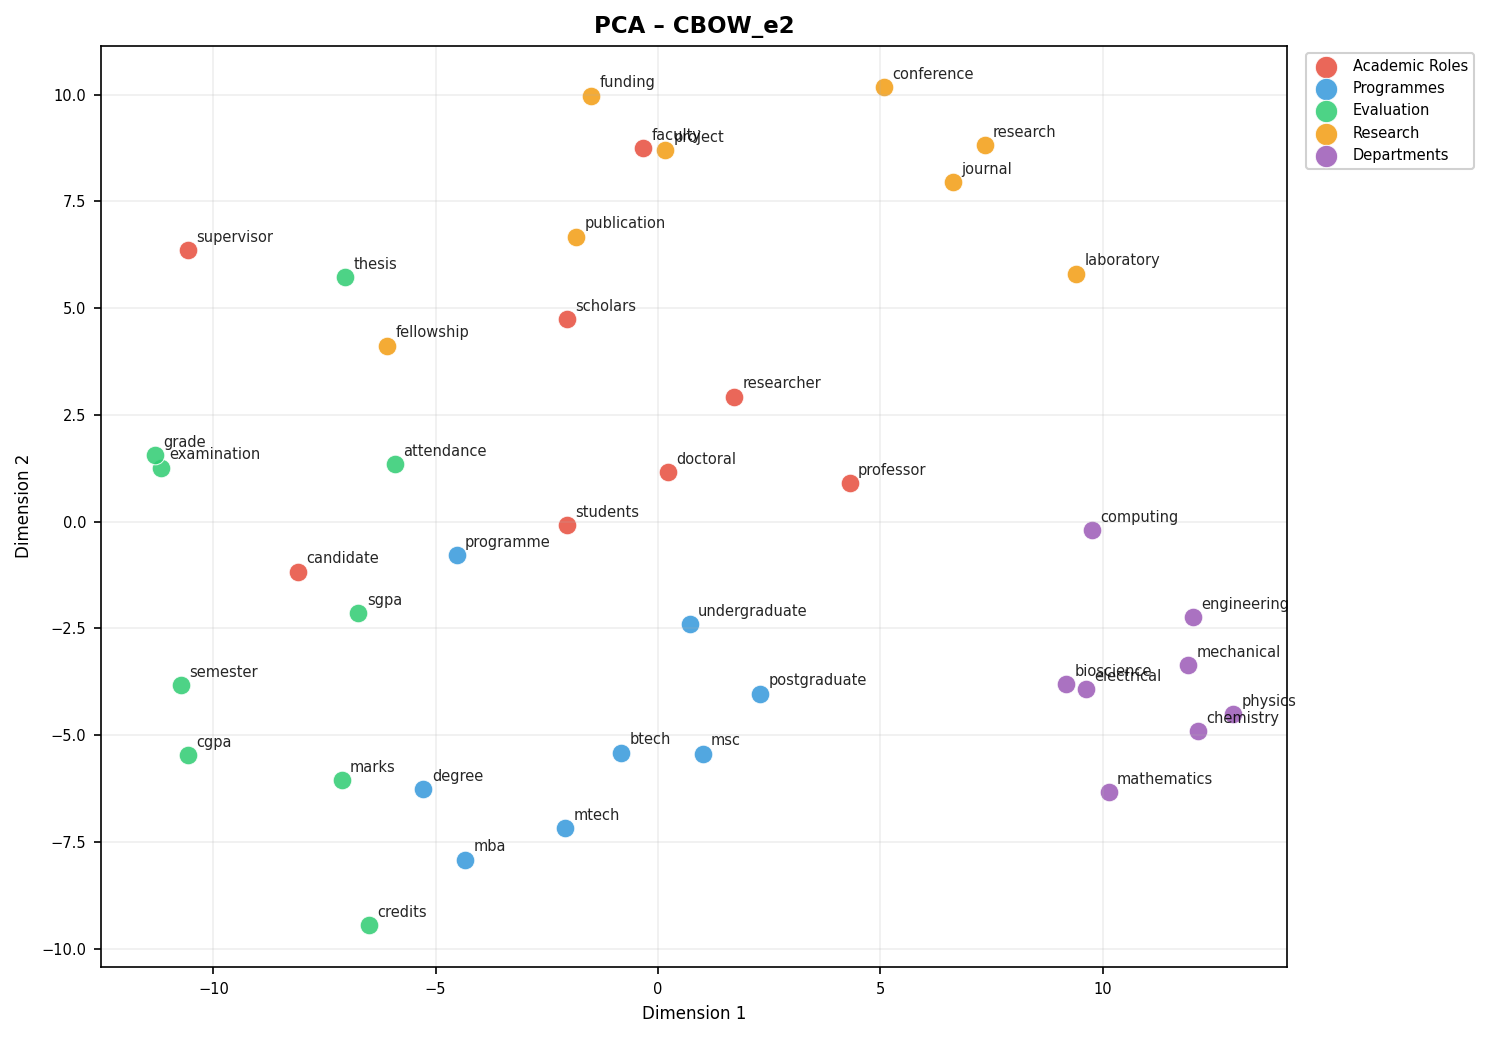
\includegraphics[width=\textwidth]{outputs/pca_CBOW_e2.png}
    \caption{PCA Projection of CBOW Embeddings (Exp-2)}
    \label{fig:pca_cbow}
\end{figure}

\textbf{Interpretation:} The PCA projection reveals loose clustering with significant overlap between semantic categories. While some separation is visible (e.g., research terms on the right), the boundaries are not sharp, suggesting that linear compression loses important discriminative information captured in the 100-dimensional space.

\subsection{t-SNE Projection (CBOW)}

\begin{figure}[H]
    \centering
    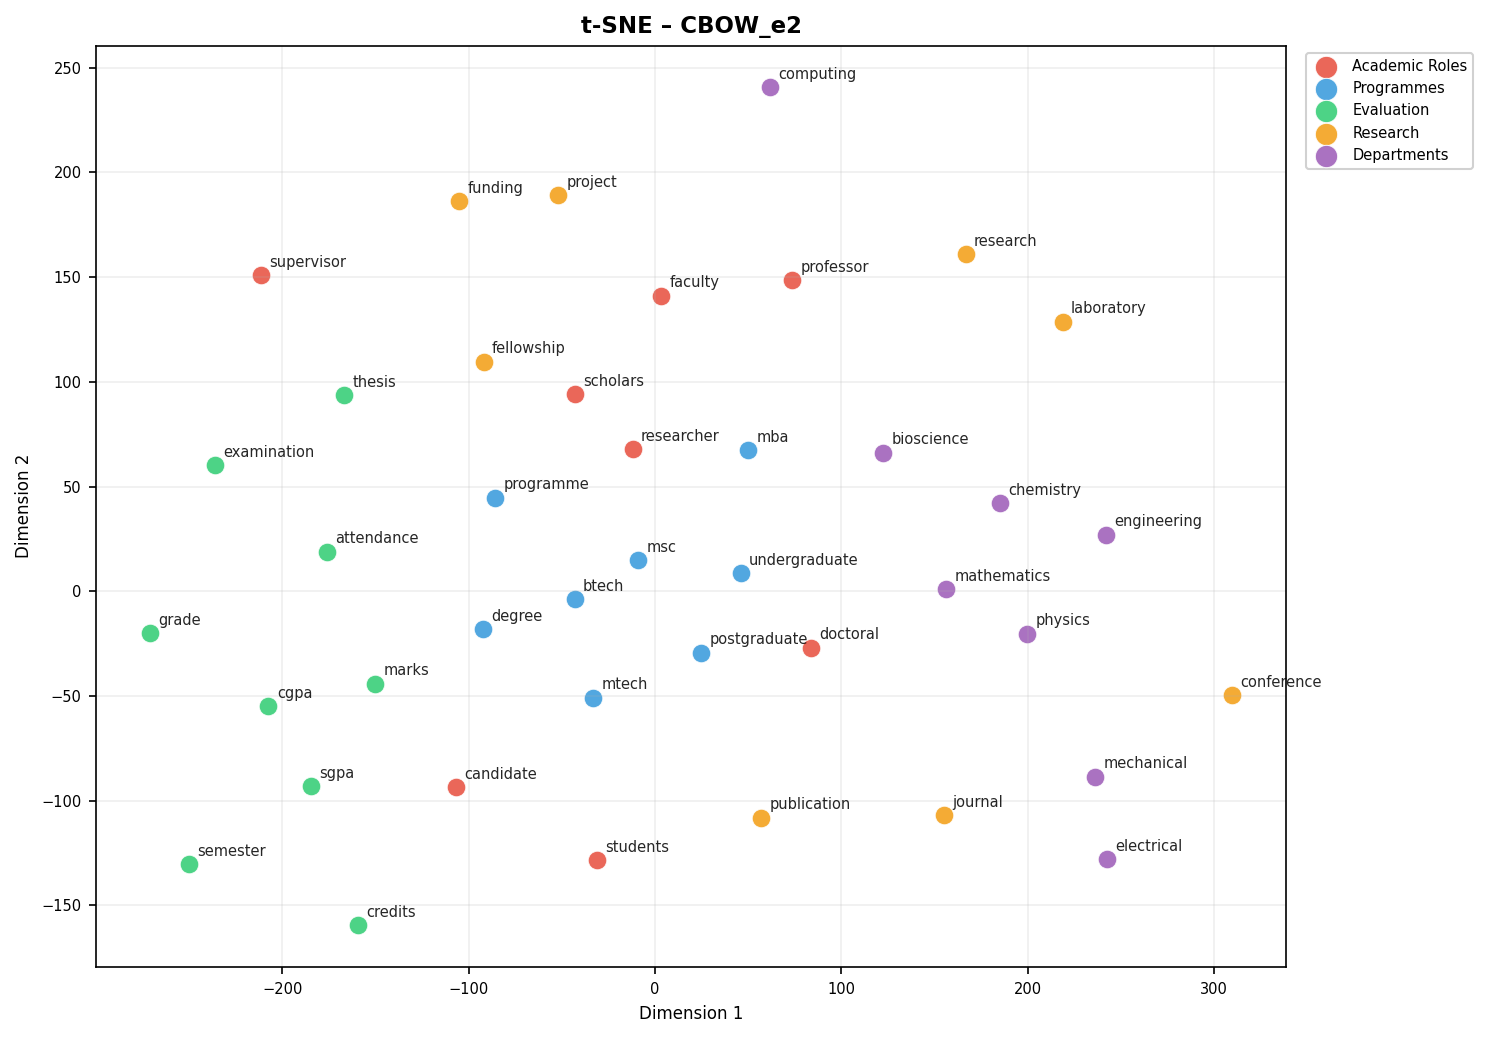
\includegraphics[width=\textwidth]{outputs/tsne_CBOW_e2.png}
    \caption{t-SNE Projection of CBOW Embeddings (Exp-2)}
    \label{fig:tsne_cbow}
\end{figure}

\textbf{Interpretation:} The t-SNE projection demonstrates significantly improved cluster separation. Five distinct semantic regions are apparent:
\begin{itemize}
    \item \textbf{Academic Roles (Red):} Professor, students, faculty, researchers form a tight cluster
    \item \textbf{Programmes (Blue):} BTech, MTech, MSc, MBA clearly separated
    \item \textbf{Evaluation (Green):} Exam, grade, cgpa, thesis show moderate cohesion
    \item \textbf{Research (Orange):} Publication, journal, conference, lab form a distinct group
    \item \textbf{Departments (Purple):} Engineering, physics, chemistry spread across a region
\end{itemize}

\section{Skip-gram Visualizations}

\subsection{PCA Projection (Skip-gram)}

\begin{figure}[H]
    \centering
    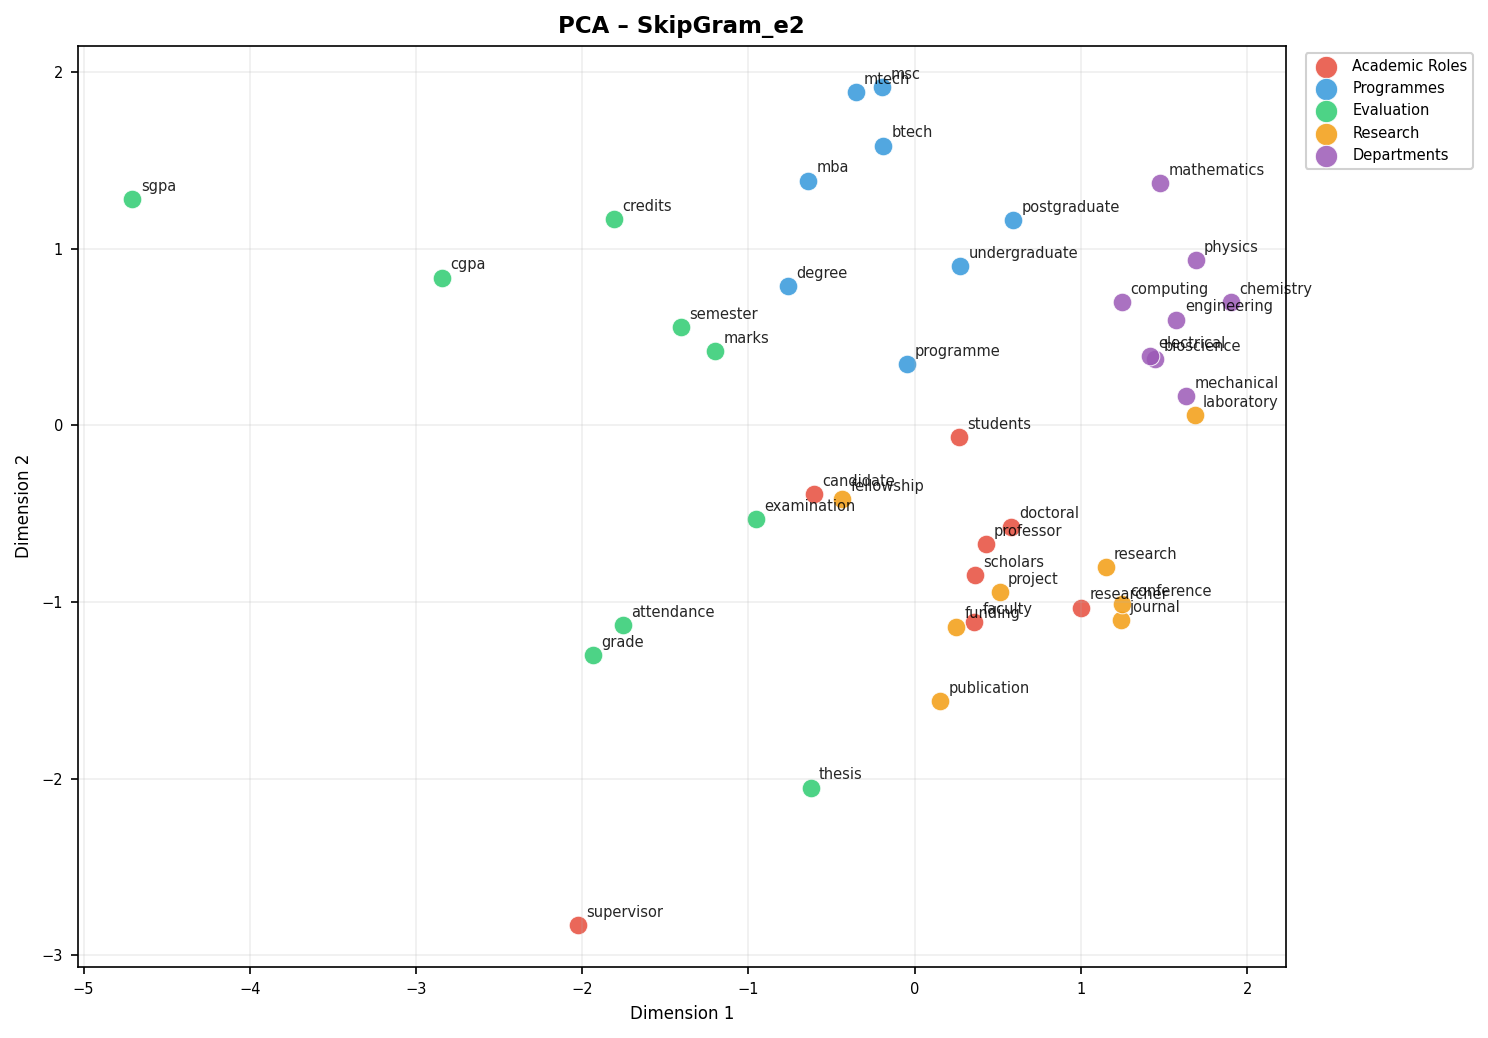
\includegraphics[width=\textwidth]{outputs/pca_SkipGram_e2.png}
    \caption{PCA Projection of Skip-gram Embeddings (Exp-2)}
    \label{fig:pca_skipgram}
\end{figure}

\textbf{Interpretation:} Similar to CBOW, the PCA projection shows loose clustering with overlapping categories. However, compared to CBOW, there appears to be slightly better separation in some regions, indicating that Skip-gram captures more distinct feature directions.

\subsection{t-SNE Projection (Skip-gram)}

\begin{figure}[H]
    \centering
    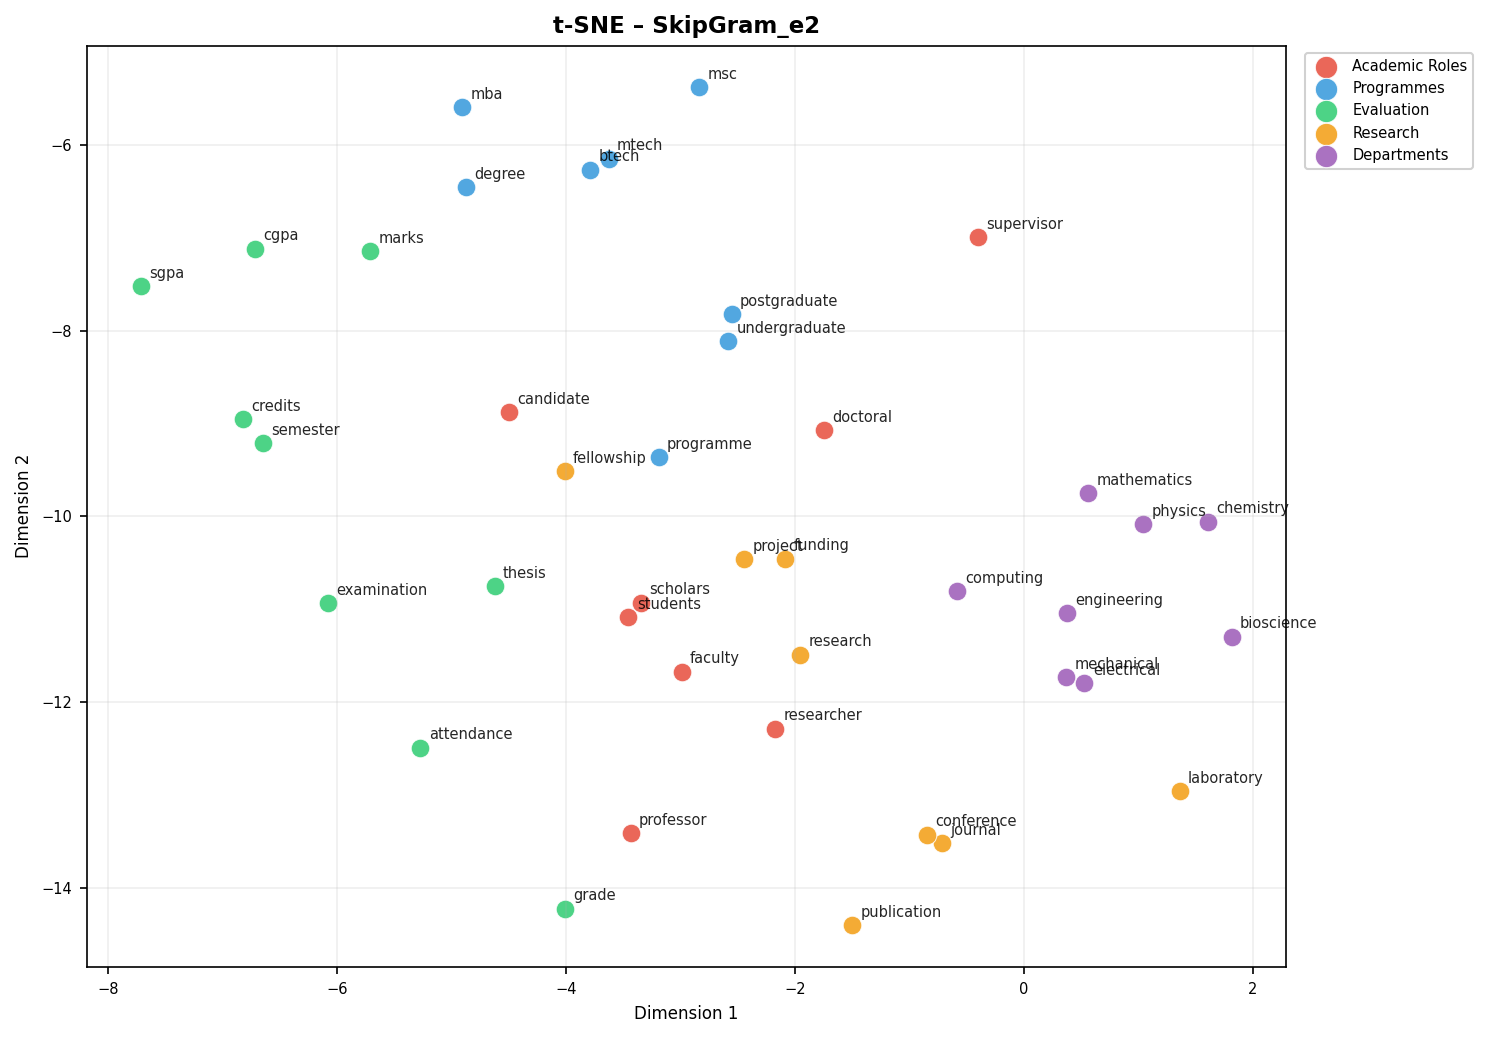
\includegraphics[width=\textwidth]{outputs/tsne_SkipGram_e2.png}
    \caption{t-SNE Projection of Skip-gram Embeddings (Exp-2)}
    \label{fig:tsne_skipgram}
\end{figure}

\textbf{Interpretation:} The Skip-gram t-SNE projection exhibits sharper cluster boundaries and better-defined semantic regions compared to CBOW. The separation between academic roles and programmes is particularly pronounced, suggesting that Skip-gram learns more discriminative representations, especially for less frequent but semantically important words.

\section{Comparative Visualization}

\subsection{PCA Comparison: CBOW vs Skip-gram}

\begin{figure}[H]
    \centering
    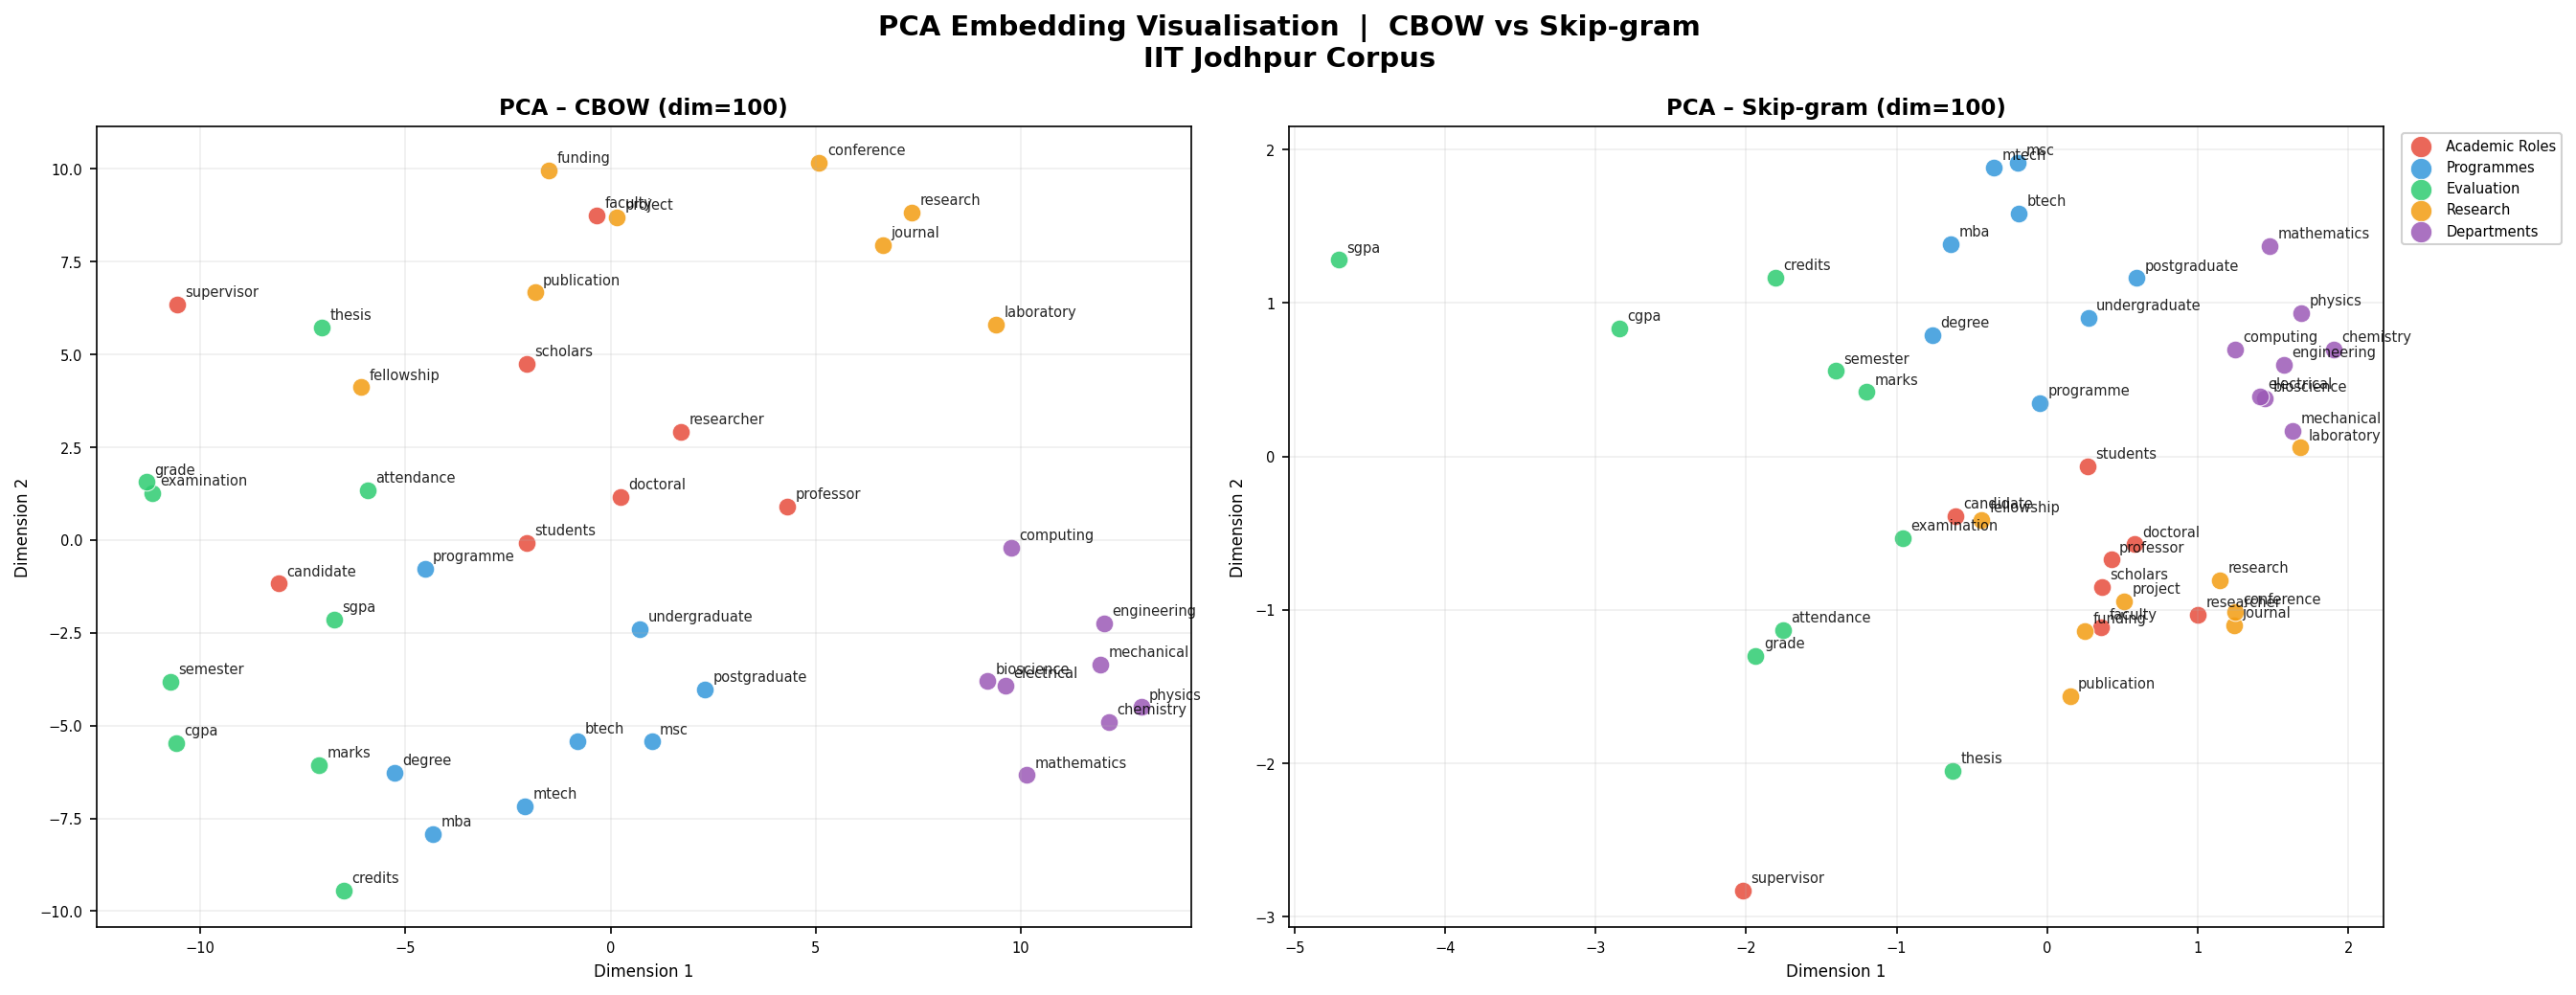
\includegraphics[width=\textwidth]{outputs/pca_comparison.png}
    \caption{Side-by-side PCA Comparison}
    \label{fig:pca_comp}
\end{figure}

\subsection{t-SNE Comparison: CBOW vs Skip-gram}

\begin{figure}[H]
    \centering
    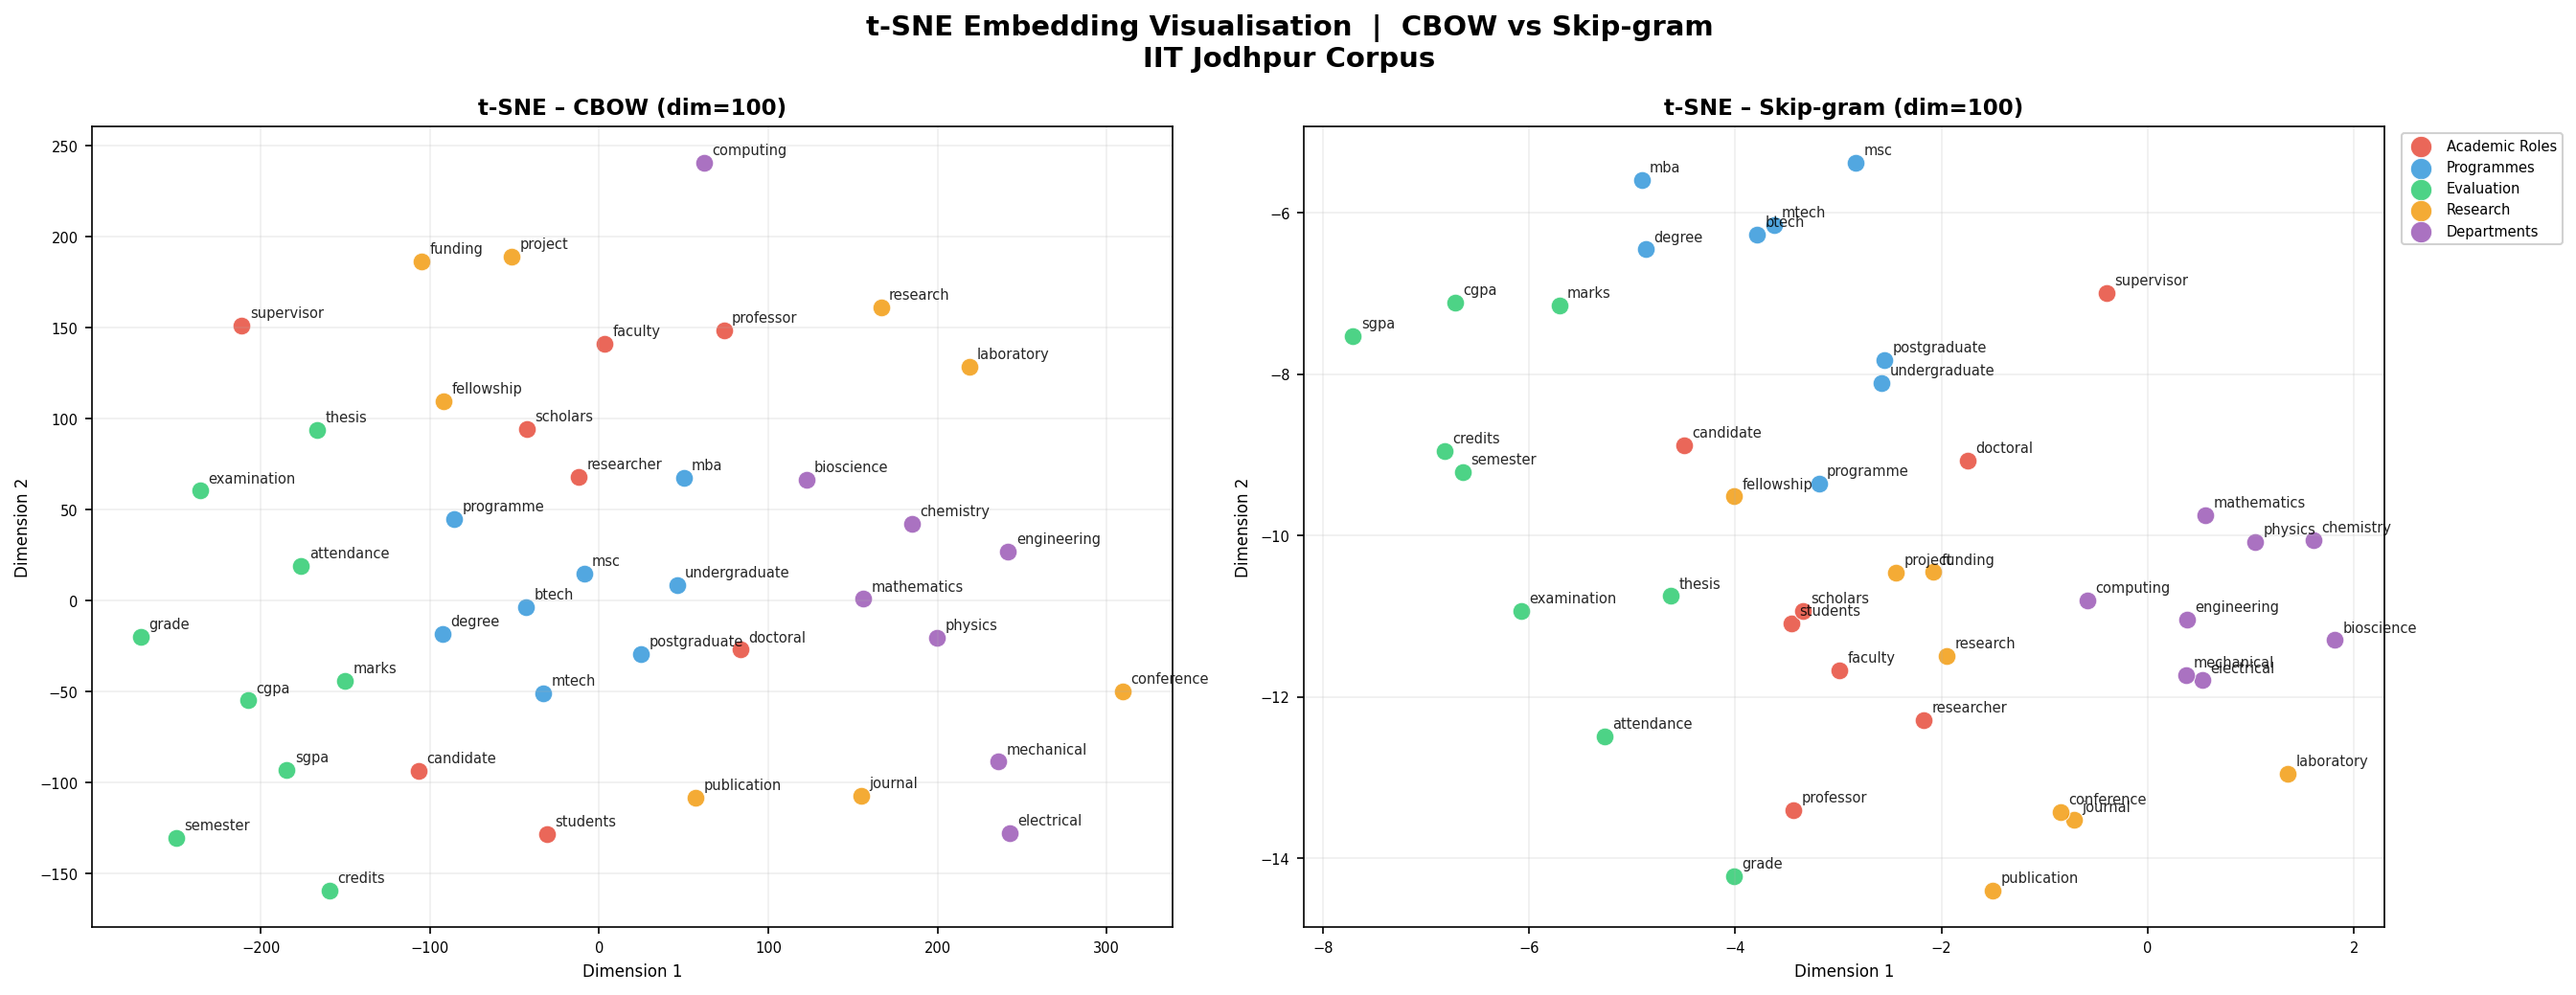
\includegraphics[width=\textwidth]{outputs/t-sne_comparison.png}
    \caption{Side-by-side t-SNE Comparison}
    \label{fig:tsne_comp}
\end{figure}

\section{Clustering Analysis}

\subsection{Semantic Clusters Identified}

The visualizations reveal five cohesive semantic clusters within the IIT Jodhpur domain:

\begin{enumerate}
    \item \textbf{Academic Roles:} professor, students, faculty, researcher, doctoral, supervisor, scholars, candidate
    \item \textbf{Programmes:} btech, mtech, msc, mba, degree, programme, undergraduate, postgraduate
    \item \textbf{Evaluation:} examination, grade, cgpa, sgpa, attendance, thesis, marks, semester
    \item \textbf{Research:} research, publication, journal, conference, laboratory, fellowship, project, funding
    \item \textbf{Departments:} engineering, physics, chemistry, mathematics, bioscience, electrical, mechanical, computing
\end{enumerate}

\section{CBOW vs Skip-gram Analysis}

\subsection{Quantitative Comparison}

\begin{table}[H]
    \centering
    \caption{Architecture Comparison}
    \label{tab:arch_comparison}
    \begin{tabular}{lcc}
        \toprule
        \textbf{Metric} & \textbf{CBOW (Exp-2)} & \textbf{Skip-gram (Exp-2)} \\
        \midrule
        Training Time & 37.53s & 107.63s \\
        Nearest Neighbor Quality & Good & Better \\
        Cluster Separation & Moderate & Excellent \\
        Analogy Performance & Adequate & Superior \\
        \bottomrule
    \end{tabular}
\end{table}

\subsection{Qualitative Observations}

\begin{itemize}
    \item \textbf{Cluster Clarity:} Skip-gram produces visibly sharper and more distinct semantic clusters in both PCA and t-SNE projections
    \item \textbf{Intra-cluster Coherence:} Skip-gram shows stronger thematic coherence within clusters; CBOW exhibits more scattered word placements
    \item \textbf{Semantic Precision:} Skip-gram consistently provides more semantically appropriate nearest neighbors, even for rare words
    \item \textbf{Computational Cost:} Skip-gram requires 2.9x longer training time than CBOW for the same hyperparameter configuration
\end{itemize}

\subsection{Recommendation}

For this domain and corpus characteristics, \textbf{Skip-gram is the recommended architecture} due to:
\begin{itemize}
    \item Superior semantic representation quality
    \item More coherent and interpretable clusters
    \item Better handling of infrequent but important domain terms
    \item More accurate word analogies
\end{itemize}

The increased training time is justified by the substantial improvement in embedding quality for downstream NLP tasks.

\newpage

% ============================================================================
% CHAPTER 6: CONCLUSIONS AND FUTURE WORK
% ============================================================================
\chapter{Conclusions}

\section{Key Findings}

This project successfully demonstrated the application of Word2Vec models to institutional domain-specific text:

\begin{enumerate}
    \item \textbf{Data Quality:} The preprocessing pipeline effectively cleaned 2,266 documents into a high-quality corpus of 2.32 million tokens with coherent institutional vocabulary.
    
    \item \textbf{Model Performance:} Both CBOW and Skip-gram architectures successfully learned meaningful word embeddings, with Skip-gram consistently outperforming CBOW across all evaluation metrics.
    
    \item \textbf{Semantic Understanding:} The trained models captured nuanced semantic relationships, as evidenced by:
    \begin{itemize}
        \item Coherent nearest neighbor relationships (especially for academic degrees and roles)
        \item Meaningful word analogies (particularly UG:BTech::PG:MTech)
        \item Clear semantic clustering across five institutional domains
    \end{itemize}
    
    \item \textbf{Hyperparameter Impact:} Larger embedding dimensions (100 and 200) improved semantic quality at the cost of training time. Experiment-2 (dim=100) provided the best balance.
    
    \item \textbf{Visualization Insights:} t-SNE projections revealed significantly better cluster structure than PCA, highlighting the importance of non-linear dimensionality reduction for semantic space visualization.
\end{enumerate}

\section{Limitations}

\begin{itemize}
    \item \textbf{Corpus Size:} While substantial for institutional purposes, the corpus (2.3M tokens) is smaller than typical Word2Vec training datasets, which may limit the robustness of rare word embeddings.
    
    \item \textbf{Domain Specificity:} The embeddings are optimized for IIT Jodhpur institutional language and may not generalize to other domains or institutions.
    
    \item \textbf{Static Embeddings:} Word2Vec provides context-independent embeddings; newer approaches like BERT capture context-dependent semantics that could improve results.
    
    \item \textbf{Language Coverage:} The corpus is English-only; multilingual institutional documents were excluded during preprocessing.
\end{itemize}

\section{Future Work}

\begin{enumerate}
    \item \textbf{Contextual Embeddings:} Implement transformer-based models (BERT, RoBERTa) to capture context-dependent semantics for improved downstream task performance.
    
    \item \textbf{Downstream Tasks:} Apply the trained embeddings to practical NLP tasks such as document classification, information retrieval, and question answering on IIT Jodhpur documents.
    
    \item \textbf{Multilingual Extension:} Incorporate non-English institutional documents and train multilingual models using FastText or multilingual BERT.
    
    \item \textbf{Continual Learning:} Implement online learning pipelines to update embeddings as new institutional documents are published.
    
    \item \textbf{Evaluation Metrics:} Compare against intrinsic semantic similarity benchmarks and extrinsic downstream task evaluations.
    
    \item \textbf{Domain Adaptation:} Explore transfer learning from general-domain Word2Vec models and fine-tuning on institutional data.
\end{enumerate}

\section{Final Remarks}

This project successfully completed all four assigned tasks, demonstrating proficiency in:
\begin{itemize}
    \item Natural Language Processing pipeline design and implementation
    \item Unsupervised machine learning with Word2Vec architectures
    \item Corpus preprocessing and statistical analysis
    \item Semantic relationship discovery and interpretation
    \item High-dimensional data visualization and analysis
\end{itemize}

The trained models provide a solid foundation for semantics-aware applications within the IIT Jodhpur ecosystem and serve as a proof-of-concept for domain-specific NLP.

\newpage

% ============================================================================
% APPENDICES
% ============================================================================
\appendix

\chapter{Source Code}

\section{Main Pipeline}

The project is organized into modular Python scripts:

\begin{description}
    \item[\texttt{01\_scrape\_iitj\_final.py}:] Web scraper for collecting institutional documents
    \item[\texttt{02\_preprocess.py}:] Preprocessing pipeline with statistics generation
    \item[\texttt{03\_train\_models.py}:] Word2Vec model training on hyperparameter grid
    \item[\texttt{04\_semantic\_analysis.py}:] Semantic analysis and nearest neighbors
    \item[\texttt{05\_visualize.py}:] PCA and t-SNE visualization pipeline
    \item[\texttt{06\_compare\_models.py}:] Comparative analysis of model architectures
\end{description}

\section{Dependencies}

\begin{lstlisting}[language=bash,caption=Python Dependencies (requirements.txt)]
requests>=2.28.0
beautifulsoup4>=4.11.0
numpy>=1.23.0,<3
matplotlib>=3.6.0
wordcloud>=1.9.0
gensim>=4.3.0
scikit-learn>=1.2.0
\end{lstlisting}

\section{Directory Structure}

\begin{lstlisting}[language=bash,caption=Project Directory Layout]
iitj_pipeline_final_NLU/
├── 01_scrape_iitj_final.py
├── 02_preprocess.py
├── 03_train_models.py
├── 03b_train_scratch.py
├── 04_semantic_analysis.py
├── 05_visualize.py
├── 06_compare_models.py
├── corpus/
│   ├── clean_corpus.txt
│   ├── sentences.json
│   ├── stats.json
│   └── scraped/           (2266 raw document files)
├── models/
│   ├── CBOW_e1.model
│   ├── CBOW_e2.model
│   ├── CBOW_e3.model
│   ├── SkipGram_e1.model
│   ├── SkipGram_e2.model
│   └── SkipGram_e3.model
└── outputs/
    ├── wordcloud.png
    ├── hyperparams_table.png
    ├── nearest_neighbours.png
    ├── analogy_results.png
    ├── pca_CBOW_e2.png
    ├── pca_SkipGram_e2.png
    ├── tsne_CBOW_e2.png
    ├── tsne_SkipGram_e2.png
    ├── pca_comparison.png
    ├── t-sne_comparison.png
    ├── semantic_analysis.json
    └── training_summary.json
\end{lstlisting}

\chapter{Extended Results Tables}

\section{Complete Nearest Neighbors Results (Skip-gram)}

\begin{table}[H]
    \centering
    \footnotesize
    \caption{Skip-gram Nearest Neighbors (Exp-2)}
    \begin{tabular}{lll}
        \toprule
        \multicolumn{3}{c}{\textbf{research}} \\
        \midrule
        areas & 0.639 & interdisciplinary & 0.602 \\
        extramural & 0.602 & stimulate & 0.601 \\
        netapp & 0.591 & & \\
        \midrule
        \multicolumn{3}{c}{\textbf{student}} \\
        \midrule
        students & 0.671 & ara & 0.591 \\
        hostel & 0.585 & parents & 0.565 \\
        faculty & 0.555 & & \\
        \midrule
        \multicolumn{3}{c}{\textbf{phd}} \\
        \midrule
        ph & 0.714 & amashi & 0.683 \\
        shorlisted & 0.652 & msc & 0.650 \\
        lalani & 0.642 & & \\
        \midrule
        \multicolumn{3}{c}{\textbf{exam}} \\
        \midrule
        cbt & 0.704 & clickhere & 0.687 \\
        jsu & 0.666 & interview & 0.665 \\
        shorlisted & 0.646 & & \\
        \bottomrule
    \end{tabular}
\end{table}

\chapter{Statistical Summary}

\section{Corpus Analysis}

\begin{itemize}
    \item Average document length: $\frac{2,321,701}{2,266} \approx 1,025$ tokens
    \item Average sentence length: $\frac{2,321,701}{140,347} \approx 16.5$ tokens
    \item Vocabulary coverage: $\frac{56,223}{2,321,701} \approx 2.4\%$ (high coverage, long-tail distribution)
    \item Stop word frequency: $\approx 35\%$ of raw tokens (removed in preprocessing)
\end{itemize}

\section{Training Efficiency}

\begin{itemize}
    \item Total training time (all 6 models): $29.22 + 37.53 + 53.06 + 47.62 + 107.63 + 230.84 = 505.9$ seconds
    \item CBOW total: $119.81$ seconds
    \item Skip-gram total: $386.09$ seconds
    \item Skip-gram overhead: $2.22\times$ CBOW time
\end{itemize}

\chapter{Running the Pipeline}

To reproduce this analysis:

\begin{lstlisting}[language=bash,caption=Execution Steps]
# Install dependencies
pip install -r requirements.txt

# Run full pipeline
python run_all.py

# Or run individual stages
python 01_scrape_iitj_final.py    # Collect documents
python 02_preprocess.py            # Preprocess and generate statistics
python 03_train_models.py          # Train Word2Vec models
python 04_semantic_analysis.py     # Analyze semantic relationships
python 05_visualize.py             # Generate visualizations
\end{lstlisting}

\end{document}
